\chapter{User Interface}
\label{chap:UI}

\section{Design}

\begin{figure}[h]
    \centering
    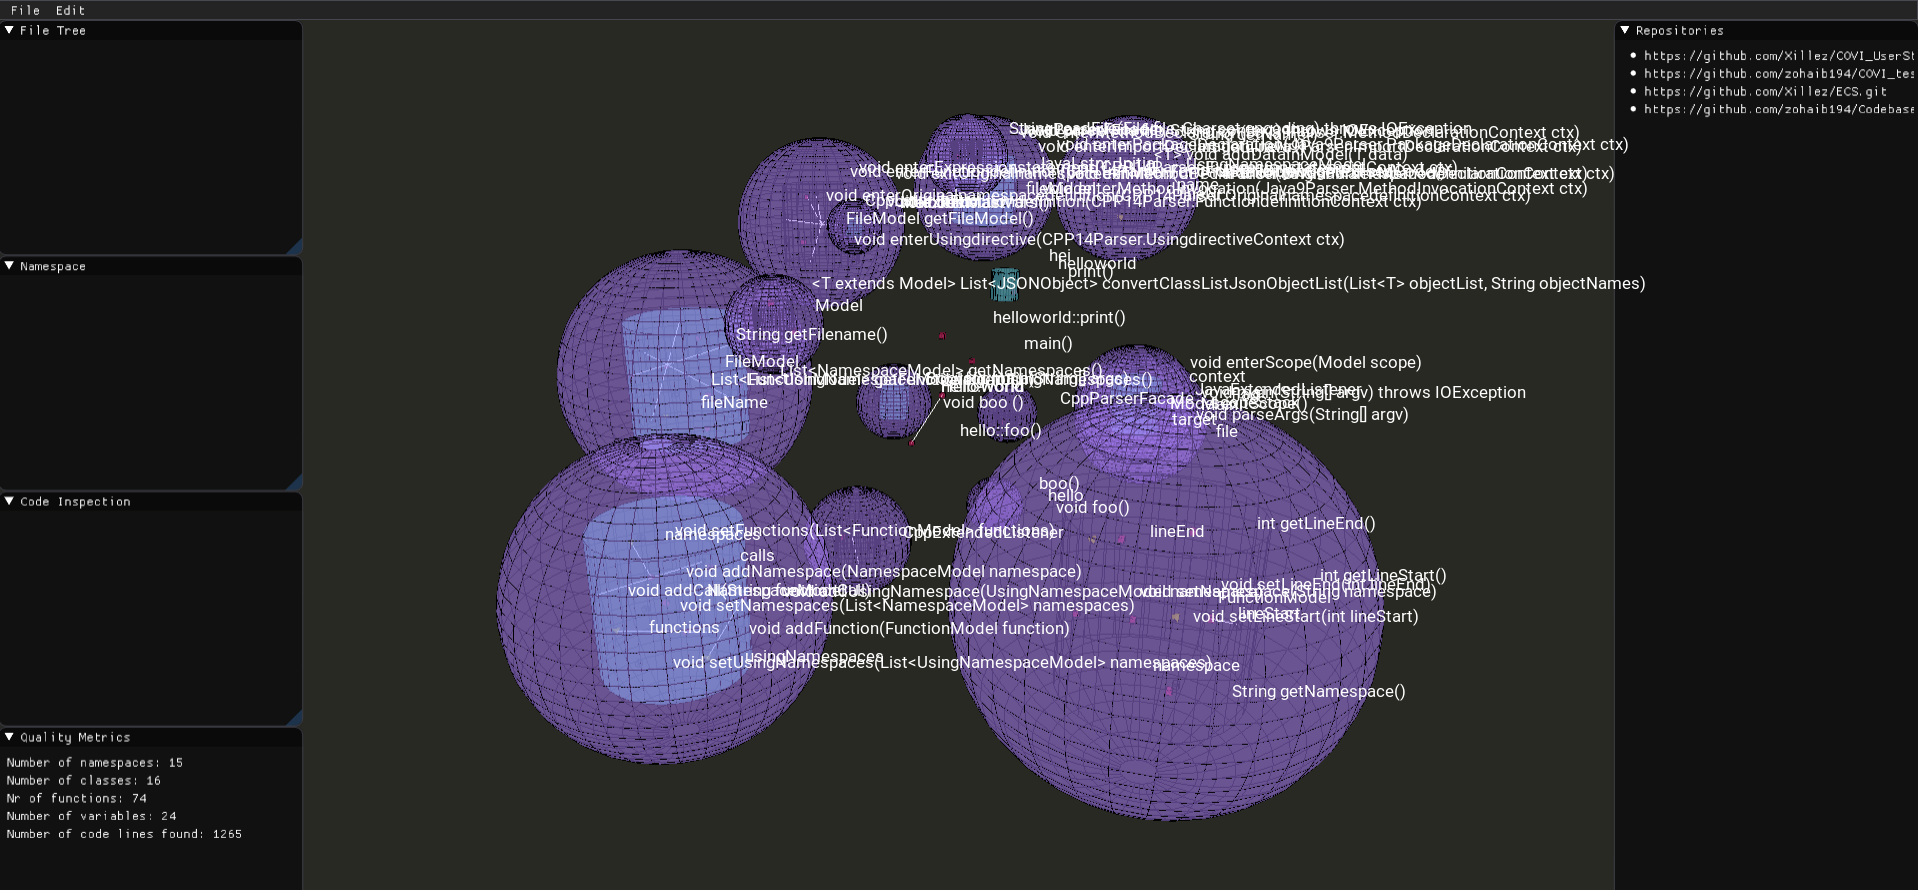
\includegraphics[width=\textwidth]{inc/images/COVI_Visualization.png}
    \caption{Final UI layout.}
    \label{fig:finalui}
\end{figure}
\newglossaryentry{tensorflow}{name={Tensorflow}, description={An end-to-end open source platform for machine learning \cite{tensorflow}}}

The initial \gls{ui} concept shown in appendix \ref{app:initialConcept}, was presented to product owner during the second meeting to visualize how the team had intended to design layout of the system. Product owner was pleased by the looks of the system and approved it.

\gls{tensorflow} visualization was an inspiration because it deals with concepts like AI and big data, which have quite understandable and readable ways to represent a big data set through graphs. The team wanted an intuitive way of visualizing the data structure along with keeping the concepts like loosely or highly coupled relationships. Therefore the \gls{tensorflow} representation seemed a perfect fit for this problem.

The left side of figure \ref{app:initialConcept}, was meant to show project related data such as file structure, namespaces, implementation and quality metrics. Whilst the right side shows project independent data, such as repositories registered in the system for easy switching between them. 

The final \gls{ui} layout is shown in figure \ref{fig:finalui}.